%%%%%%%%%%%%%%%%%%%%%%%%%%%%%%%%%%%%%%%%%%%%%%%%%%%%%%%%%%%%%%%%%%%%%%%%%%%%%%%%
% This covers the problem analysis portion of the thesis
%
%%%%%%%%%%%%%%%%%%%%%%%%%%%%%%%%%%%%%%%%%%%%%%%%%%%%%%%%%%%%%%%%%%%%%%%%%%%%%%%%

\chapter{Problem and Analysis}
This chapter proposes our alternative approach for navigating a large body of
text. In particular, we introduce our dataset and problem domain: exploring 
vehicle complaint reports for reliability and safety analysis. We introduce our
goals and our requirement gathering process. Lastly we take a closer look at
our dataset records and specify the dimensions we want to visualize to support
our goals.

    % ===== Figure =====
	\begin{figure}
       \begin{center} 
       \begin{tabular}{c}
       \framebox[1\width ]{
       \begin{tabular}{l}
       The car is wandering sideways and you have to really control and \\
       focus on keeping the wheel straight to stay on lane. The best way \\
       to describe it is like you are always driving on windy weather \\
       with severe wind gusts. This happens on highway, with a speed of 60 \\
       MPH or higher. The assistant service manager said it could be the \\
       wheel alignment but after they aligned it and checked it, the problem \\
       remains. I live in an area where we get significant amount of snow \\
       during winter and I am afraid of my safety because of this problem. \\
       \end{tabular}
       } \\
       \end{tabular}
       \end{center}	
 	   \caption{An example of a complaint summary}
	   \label{figure:complaint}
	\end{figure}
	% ==================

%   % ===== Figure =====
% 	\begin{figure}
% 	   \centering  
% 	   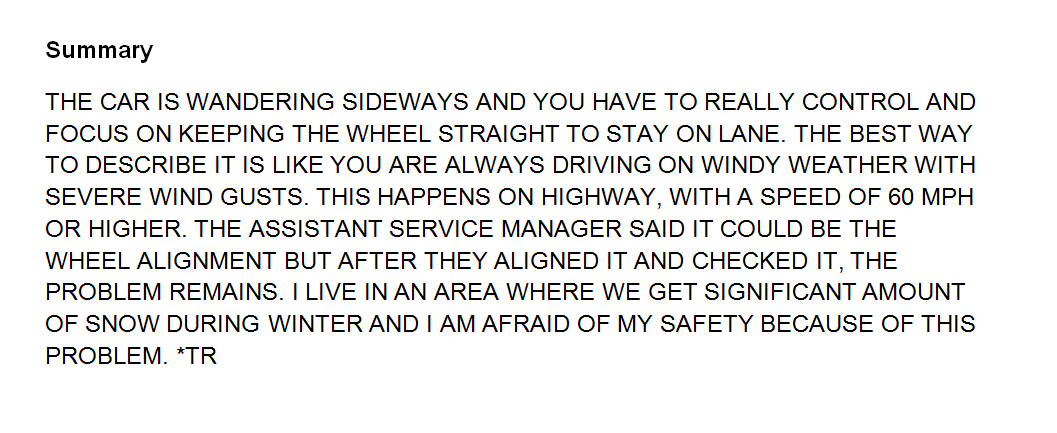
\includegraphics[width=\columnwidth]{complaint_text.png}
% 	   \caption{An example of a complaint summary}
% 	   \label{figure:complaint}
% 	\end{figure}
% 	% ==================


\section{Problem}
When it comes to navigating, exploring and querying large bodies of text,
traditional visualization techniques often approach the problem from an abstract
perspective. These techniques explores the context of words in the sentence of
the documents, for example Word Tree \cite{Wattenberg2008} allows people to
explore the most frequently occurring sentence structures within a document.
Other types of visualization looks at summarizing the underlying text, popular 
visualizations on the web today such as tag-clouds and word-cloud emphasize
the most frequently occurring words or phrases, thus revealing possible themes in
the text. Still, other techniques looks at the language semantics, for example 
DocuBurst \cite{COL2009a} spatially organize words based on the ``IS-A'' relationship.

Looking at the underlying semantics helps us understanding the content and 
themes in the text documents. However, there is another type of word context 
that is not fully explored in the visualization community. Within any text 
document which describes physical objects, each word that describes a 
tangible object has relation to its physical, real world counterpart. The 
entities also have relation to each other in terms of their respective 
spatial positions. For example, the sentence ``Automatic door locks when 
used, will not release from any of the four doors when engine is turned off.'' 
contains not only a co-occurrence relationship among the entities ``door'' and 
``engine'', but also relates to where the doors and engine are located on a 
real world automobile.

% Revealing these spatial relations of common words in text may enable new types of 
% insights and exploration techniques. By mapping physical entities onto virtual
% \threed representations it is possible to create a visualization environment
% that resembles the real world, the environment can then be explored and queried with relative ease
% due to existing familiarity of how these objects operates in real life. There are 
% many types of text that carries these sort of physically mappable vocabulary: 
% product reviews, technical manuals, maintenance logs, and our dataset: vehicle 
% defect reports.

Revealing the spatial dimensions has several benefits. Foremost, the
familiarity of the form makes the subject matter immediately recognizable
to experts and novices alike, combined with the message-carrying
capability of NPR illustrations, we argue that our approach is creates a
rich, engaging experience. Second, it is possible to conduct a different
type of data exploration: the spatial dimension allows us to explore
proximal relations and filtration by spatial volumes, possibly allowing
new insights to be formed.

So far, we are not aware of any exploratory visualizations which approach text
visualization by visualizing the real-world spatial context of the words in
text. Thus, our work looks at revealing these real world relations in a manner
that is useful for conducting text-analytic activities.

Consider product quality reports for a musical instrument. Visualizing
these report allows one to see exact location of the problems on the
3D model, for example: which valves are failing. Seeing the instrument
in physical form may promote conjectures that are less apparent
with text or abstract visualization, for example: perhaps the valves
failed because they are encased in a faulty housing. There are many
applicable datasets which carry this sort of physically mappable vocabulary:
consumer product reviews, technical manuals, and technical
support logs are examples.



\section{Use Case: Vehicle Complaint Reports}
We choose to demonstrate our approach on a dataset of vehicle complaint
reports. Each year thousands of reports are submitted to the
NHTSA database, consisting of consumer complaints, defect reports
and manufacturer recalls. Each report has fixed fields describing the
details of the incident (date, make, model, etc.), and a free-form text
field, typically containing several sentences which describe the incident
in detail, including what physical parts were damaged or broken. A sample of the
text description, which we use to drive our visualization, can be seen in Figure
\ref{figure:complaint}. Thus this data can be mined for frequency counts as
well as co-occurrence counts of car parts. All together the meta data and free
text offer a wealth of information on safety and reliability issues of
vehicles. Consumers can access this data online to support car-buying
decisions. The current interface uses a conventional search form, returning
long lists of textual results; there are no mechanisms to support
concise overviews or dynamic details-on-demand. 


 

% \subsection{Background and Requirement Gathering}
% One of the tasks for buying a vehicle is to examine the safety and reliability 
% of the vehicle. The NHTSA database offers a wealth of information to guide 
% purchasing decisions, as well as inform insurance companies and automotive 
% manufacturers about potentially serious safety and reliability concerns as reported 
% through experiences of real drivers in realistic scenarios. However, we have yet 
% to see any sophisticated ways of representing this dataset. Consumers have to
% use conventional search forms that returns a large number of amounts of textual
% results; there are no mechanism to support concise overviews or dynamic details on demand. 
% The step-by-step querying process also prevent  consumers from freely exploring 
% the data, they need to have a preconceived notion of what they want to look for, 
% thus likely prevent any type of unexpected discoveries.
% 
% On the other end of the spectrum, there exist consumer product website such as 
% Consumer Reports\footnote{http://www.consumerreports.org/} and
% Edmunds\footnote{http://www.Edmunds.com}. These website provide reviews and
% linear scale ratings for different types of vehicles, but these ratings seldom
% provide details and in-depth analysis. In other words, the ratings are too
% coarsely grained. Yet another issue with these websites is that they are
% typically targeted at newer vehicle models, as such, it can be difficult to look
% up and compare ratings between new and old models.
 
 
% \section{Tasks}
% While our data is temporal in nature and new 
% reports are constantly being added, our system is not, strictly speaking, a 
% real-time system that consumes streaming text data. Our system consume data in 
% batches, and to our knowledge, there are no known external facing API available 
% for monitoring updates. Having said that, our system share many of the same 
% concern as real time text streaming applications. Rohrdanz \etal
% \cite{ROH2011a} outline seven important tasks analytical tasks for working with
% text streams which we found to be suitable for our problem domain. These
% includes monitoring, decision making, change/trend detection, event tracking,
% historical retrieval, exploration and situational awareness.
% 
% For the purpose of analyzing vehicle defect reports, and for an audience of prospective 
% car/used-car buyers, some of the vital tasks are:
% \begin{itemize}[noitemsep]
%   \item Decision Making: ``Which vehicle should I buy?''
%   \item Historical Retrieval: ``Are there any major concerns with vehicle X over
%   the last 5 years?''
%   \item Exploration: ``How does vehicle X compare to other vehicles in the same
%   category?''
% \end{itemize}
% 
% From the perspective of an assurance engineer or incident investigator, the
% tasks may be:
% \begin{itemize}[noitemsep]
%   \item Monitoring: ``Are there any new complaints relating to vehicles of make
%   Y?''
%   \item Decision Making: ``Are there enough reports and evidences to warrant a
%   full scale investigation or a recall?''
%   \item Change and Trend Detection: ``For this type of vehicle, are the rate of
%   complaints per month increasing or decreasing?''
%   \item Situational Awareness: ``How does reports about my vehicle compare to
%   the current state of the automobile industry''
% \end{itemize}
% 
% In our design, we aim to create an application which aims to support these users
% and user tasks as they analyze these complaint reports. We take the view of the 
% consumer as the primary stakeholder. Thus, our goal is to provide text-analytic 
% visualization for helping consumers understand and explore vehicle safety issues, 
% which in turn will affect their purchasing decisions

\subsection{Requirements and Tasks}
In order to derive concrete requirements for our design, we needed to determine
the considerations which are most important to a consumer, whether for
purchasing for problem investigation.

We start our initial requirement gathering by looking at websites dedicated to 
vehicle owners and potential car buyers, our sources include expert columns, 
question and answer forums, car-buying tips and product rating websites such 
as Consumer Reports\footnote{http://www.consumerreports.org/} and
Edmunds\footnote{http://www.Edmunds.com}. 

Our findings revealed that, aside from the price factor, the next item people
care  about are safety and reliability.
This makes sense, purchase of a vehicle is a big investment, the vehicle itself 
needs to be reliable to be used frequently and ensure the safety of its passengers. 
In general, consumers want to know which brand/make they can trust. Other forum
posts refer to existing problems, with the owners asking whether the problem is an 
isolated event or if the issue is widely spread, this indicates a need and
willingness for detailed exploration. Car buying guides often advocate conducting thorough 
research on the vehicle and brand history, as well as leverage the experience of 
other owners. This is particularly important for used vehicles.
 
Based on these findings, we propose the following four design requirements for
our visualization prototype:
\begin{itemize}[noitemsep]
  \item R1: Provide an intuitive representation and make important items clearly
  visible;
  \item R2: Facilitate finding of trends, interesting facts and causal relations
  in the reports;
  \item R3: Allow multiple types of comparisons across different data
  dimensions;
  \item R4: Provide for reading of original complaint report text in the context
  of the visualization.
\end{itemize}

The types of tasks that we want to support are based on Rohrdanz \etal's seven
important analytical tasks for dealing with streaming data~\cite{ROH2011a}. 
Though the vehicle complaint dataset is not real-time it is temporal in nature
and shares many of the same concerns as real-time applications. The tasks are:

\begin{itemize}[noitemsep]
   \item Decision Making: Which vehicle should I buy? Are there enough
   reports and evidences to warrant a full scale investigation or a recall?
   \item Historical Retrieval: Are there any major concerns with vehicle X over the last 5 years?
   \item Exploration: How does vehicle X compare to other vehicles in the same category?
   \item Monitoring: Are there any new complaints relating to vehicles of make Y?
   \item Change and Trend Detection: For this type of vehicle, are the rate of complaints per month increasing or decreasing?
\end{itemize}


% \section{Data Dimensions}
% A typical complaint report consist of both structured and unstructured fields.
% The structured fields related to the type of vehicle and other explicitly 
% quantifiable variables relating to the incident (\eg, the odometer reading, 
% number of injuries, the incident location). The unstructured field is a
% free-form text field, it typically consist of several sentences describing the
% circumstances of the incident.
% 
% \textbf{Spatial:} Many texts contain spatial variables that can be mapped to the
% real, physical world. Sometimes these are explicitly stated, such as GPS 
% coordinates which are mapped to a specific location on earth, others, such as 
% an article about computer hardware, have implicit spatial locations in how the 
% described components are arranged with respect to each other. Visualization 
% offers a unique opportunity to gain insights about spatial patterns in a text 
% document by showing inherent spatial relations that are not apparent from looking 
% at the source text or their abstracted forms. For example, under Gestalt perception 
% of proximity, highlighted objects can naturally form clusters and other patterns 
% in \threed space, which can drive further analysis and exploration. Our spatial
% variables are the vehicle components, for example the engine, wheel and doors. 
% Like puzzle pieces, all together these component form a complete automobile.
% \threed visualization is not a trivial task, due to perceptual limitations it
% has many challenges when projected onto a \twod screen space
% \cite{WAR2004b}. However, a carefully designed \threed interface can also create a simple,
% compelling experience for people, particularly if the design goes above and beyond the 
% constraints of normal reality \cite{Shneiderman2003}.
% 
% \textbf{Time:} Time is almost omnipresent when dealing with streaming or reporting data, 
% whether it is the creation date or the timestamps within the document itself. 
% For our specific dataset, we suspect that much interesting information can be 
% gained by supporting high level activities such as seeing how a particular 
% object changes over time, and comparison of season to season statistics. Being
% able to search, compare and extrapolate trend information across time is vital for 
% understanding the underlying data, thus making time an obvious choice for our 
% visualization.
% 
% \textbf{Hierarchy:} The organizational hierarchy of the vehicle manufacturers
% (Manufacturer, Make, Model, Model Year) is an important aspect when purchasing 
% a vehicle. Consumers not only want to compare model-to-model in terms of 
% reliability and safety, they are also interested in whether the manufacturing 
% companies are producing reliable vehicles in general and how manufacture rank 
% with respect to each other. The organization hierarchy present a natural 
% progression from the most general selection down to specific models, and thus 
% supports successive refinement of queries. Note that the selection of 
% organizational hierarchy as a data dimension is a problem specific decision, 
% it does not generalize to text analytics for other domains.


